% An example document for Calmpage.
% Open this folder in Calmpage. main.tex is the root;
% the files in sections/ are read with \input.
\documentclass[11pt]{article}

\usepackage[T1]{fontenc}
\usepackage{lmodern}
\usepackage[margin=1.1in]{geometry}
\usepackage{amsmath}
\usepackage{booktabs}
\usepackage{siunitx}
\usepackage{microtype}
\usepackage{pgfplots}
\pgfplotsset{compat=1.18}
\usepackage[hidelinks]{hyperref}

\title{How Ink Spreads in Washi Paper}
\author{nogu}
\date{}

\begin{document}

\maketitle

\begin{abstract}
  A drop of sumi ink on washi paper does not stay where it
  lands. It is pulled into the fibres by capillary action
  and then keeps spreading by diffusion, leaving the soft
  edge that calligraphers call \emph{nijimi}. This note
  sketches a simple model of that spreading and shows why
  the stain grows with the square root of time.
\end{abstract}

\section{Introduction}

Washi is made from long plant fibres that are only loosely
pressed together. The gaps between them form a network of
tiny channels, and a liquid that touches the sheet is
drawn into that network at once. Sumi ink is a suspension
of fine soot in water and animal glue, so the water
travels faster than the pigment it carries.

What the eye sees is the result of two processes working
together: capillary flow, which sets how far the water
reaches, and diffusion, which blurs the pigment within the
wet area.

\section{A simple model}

Treat the sheet as a thin, uniform medium and let $c(r,t)$
be the concentration of pigment at distance $r$ from where
the drop landed. Within the wet region the pigment obeys
the diffusion equation
\begin{equation}
  \frac{\partial c}{\partial t} = D\,\nabla^2 c,
  \label{eq:diffusion}
\end{equation}
where $D$ is the diffusion coefficient of the pigment in
the paper. For a drop that deposits a mass $M$ at a single
point, the solution of~\eqref{eq:diffusion} in two
dimensions is
\begin{equation}
  c(r,t) = \frac{M}{4\pi D t}\,
           \exp\!\left(-\frac{r^2}{4 D t}\right).
  \label{eq:solution}
\end{equation}
The profile keeps its shape and only widens: its width is
set by the length $\ell(t) = \sqrt{4 D t}$.

The water front moves in the same way. For capillary flow
through channels of radius $a$, the Washburn equation
gives the distance reached after time $t$ as
\begin{equation}
  L(t) = \sqrt{\frac{\gamma\, a\, t \cos\theta}{2\eta}},
  \label{eq:washburn}
\end{equation}
with surface tension $\gamma$, contact angle $\theta$, and
viscosity $\eta$. Both lengths grow as $\sqrt{t}$, which
is why a stain spreads quickly at first and then seems to
stop.

\section{Results}

Figure~\ref{fig:profiles} plots~\eqref{eq:solution} at
three moments for $D =
\SI{0.5}{\milli\metre\squared\per\second}$. Each time the
elapsed time is multiplied by four, the stain becomes
twice as wide and its centre four times as pale.

\begin{figure}[h]
  \centering
  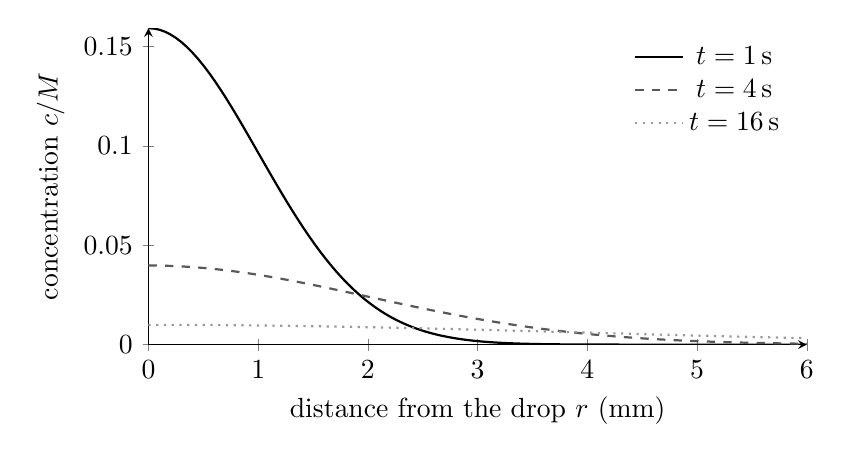
\begin{tikzpicture}
    \begin{axis}[
        width=0.82\linewidth, height=5.6cm,
        xlabel={distance from the drop $r$ (\si{\milli\metre})},
        ylabel={concentration $c / M$},
        xmin=0, xmax=6, ymin=0,
        domain=0:6, samples=120,
        axis lines=left, legend style={draw=none},
        scaled y ticks=false,
        yticklabel style={/pgf/number format/fixed},
        cycle list={{black, thick}, {black!65, thick, dashed},
                    {black!40, thick, dotted}},
      ]
      \addplot {exp(-x^2/(4*0.5*1))/(4*pi*0.5*1)};
      \addlegendentry{$t = \SI{1}{\second}$}
      \addplot {exp(-x^2/(4*0.5*4))/(4*pi*0.5*4)};
      \addlegendentry{$t = \SI{4}{\second}$}
      \addplot {exp(-x^2/(4*0.5*16))/(4*pi*0.5*16)};
      \addlegendentry{$t = \SI{16}{\second}$}
    \end{axis}
  \end{tikzpicture}
  \caption{Pigment concentration across the stain, from~\eqref{eq:solution}.}
  \label{fig:profiles}
\end{figure}

Different papers spread ink by different amounts, mostly
because their fibres leave channels of different sizes.
Table~\ref{tab:papers} lists illustrative values for three
common fibres.

\begin{table}[h]
  \centering
  \begin{tabular}{l l S[table-format=1.1]}
    \toprule
    Paper & Fibre & {Spread after \SI{10}{\second} (\si{\milli\metre})} \\
    \midrule
    Kozo      & long, coarse & 6.5 \\
    Mitsumata & fine, soft   & 4.0 \\
    Gampi     & very fine    & 2.5 \\
    \bottomrule
  \end{tabular}
  \caption{Illustrative spread for three washi fibres. The values are
    made up for this example.}
  \label{tab:papers}
\end{table}


\end{document}
